
\Problem{Arbres Fractals}

\Statement

Voleu pintar en Python arbres fractals tant xulos com aquest?

\begin{center}
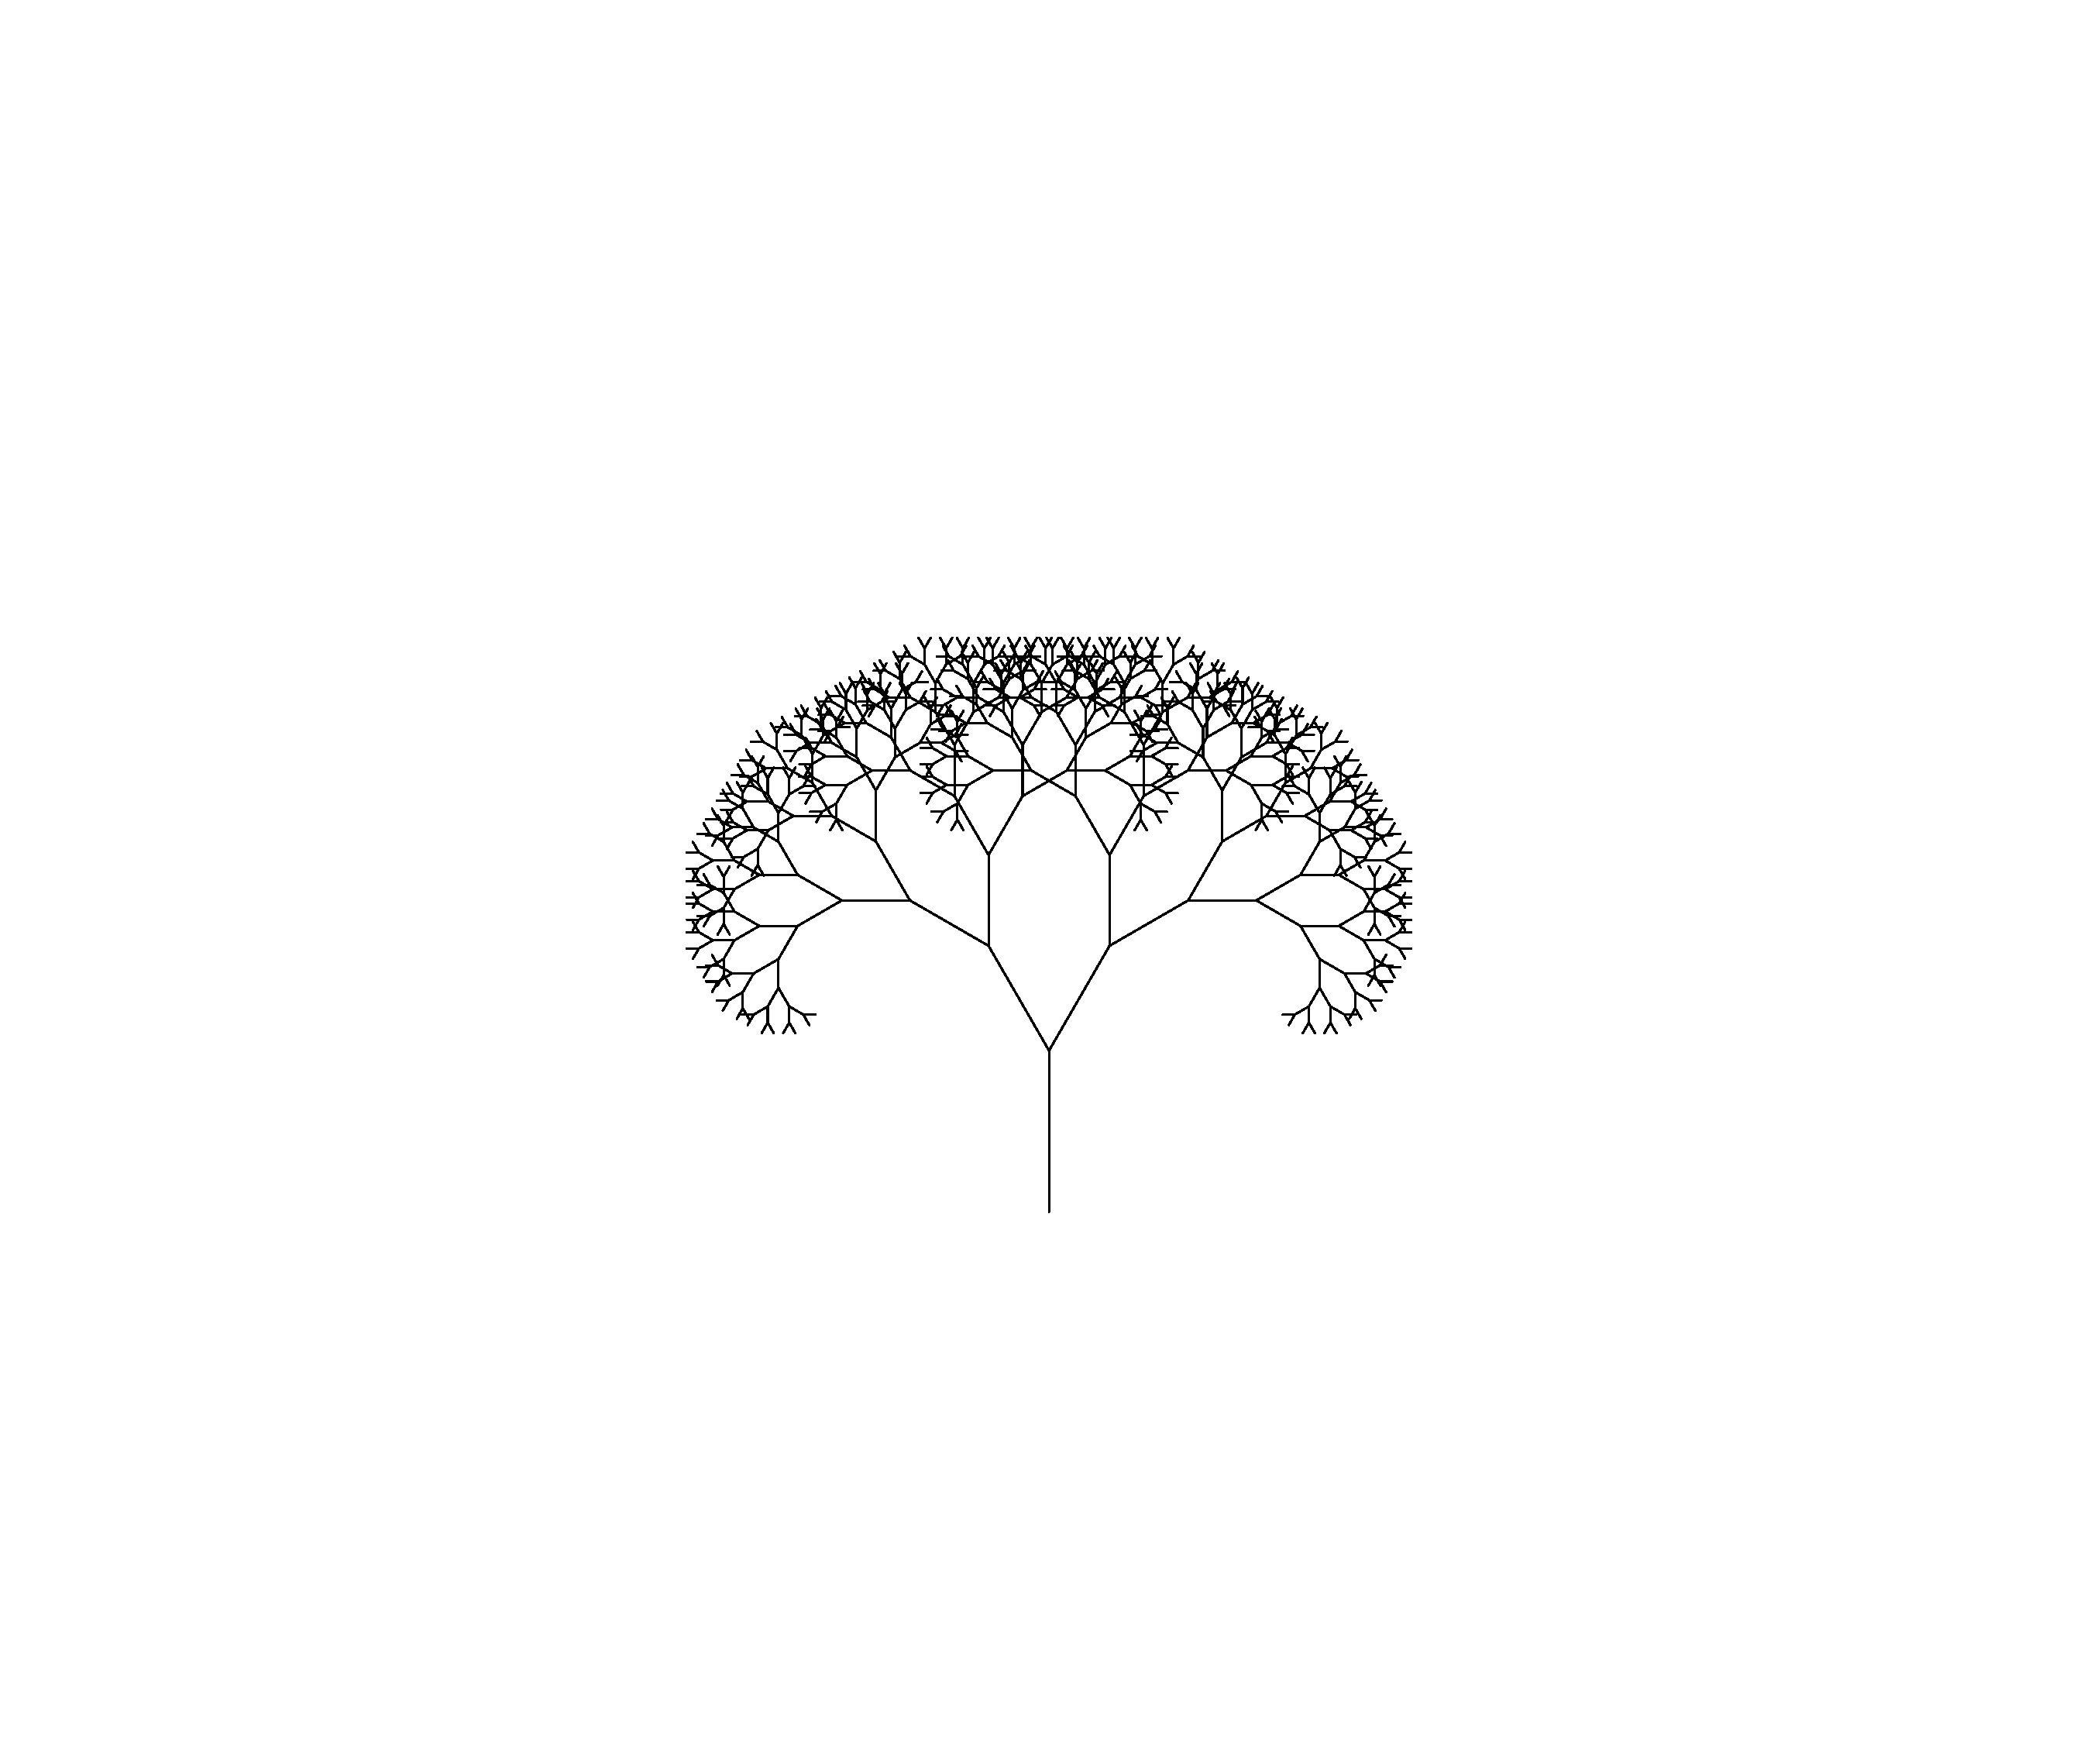
\includegraphics[trim=350 300 350 375,height=5cm]{10.eps}
\end{center}

Per pintar un arbre de $n\ge1$ nivells de mida $d$, cal pintar el seu tronc de
mida $d$, la seva branca esquerra i la seva branca dreta, ambdues com a arbres
de $n-1$ nivells i mida $\frac34 d$,  i simètriques respecte del tronc amb un
angle de $2\alpha$ graus entre elles. Un arbre de zero nivells és buit.

\bigskip

Per exemple, aquests són els arbres (de mida 100) amb 1, 2, 3, 4, 5 i 6 nivells
quan $\alpha=30$:

\begin{center}
1 ~
\fbox{

\includegraphics[trim=450 300 450 375,height=3.5cm]{1.eps}
}
\qquad
2 ~
\fbox{
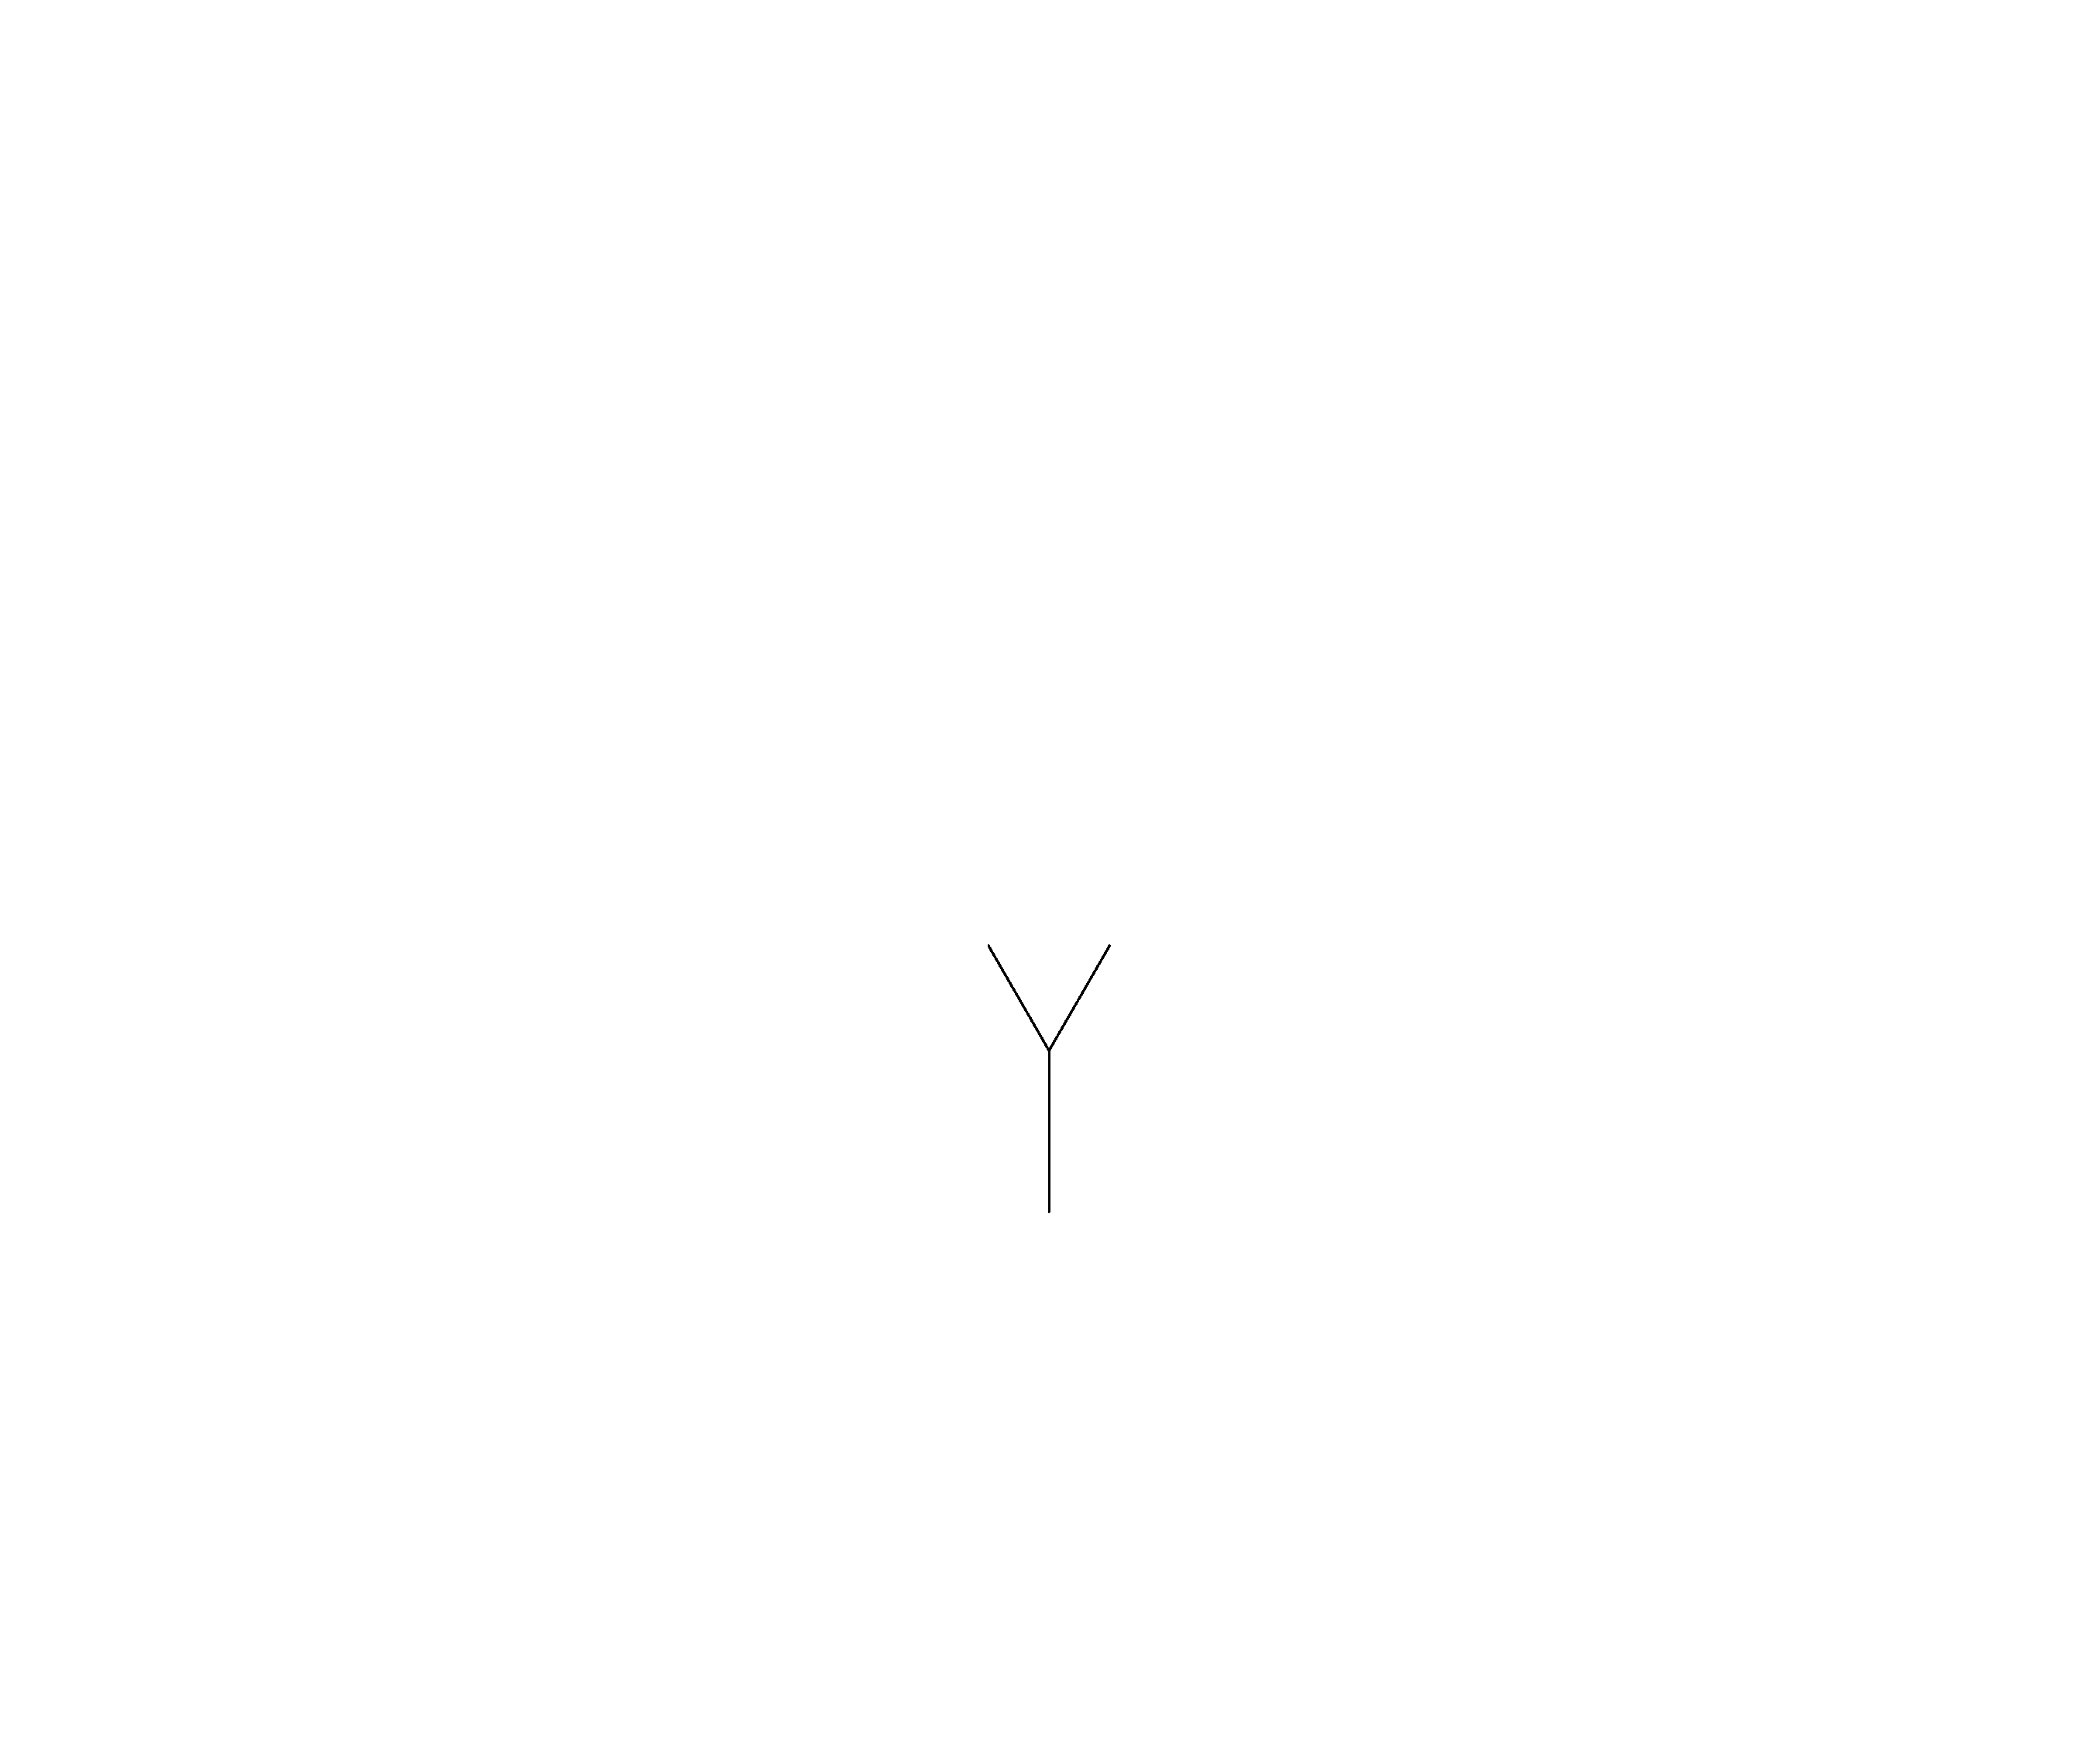
\includegraphics[trim=450 300 450 375,height=3.5cm]{2.eps}
}
\qquad
3 ~
\fbox{
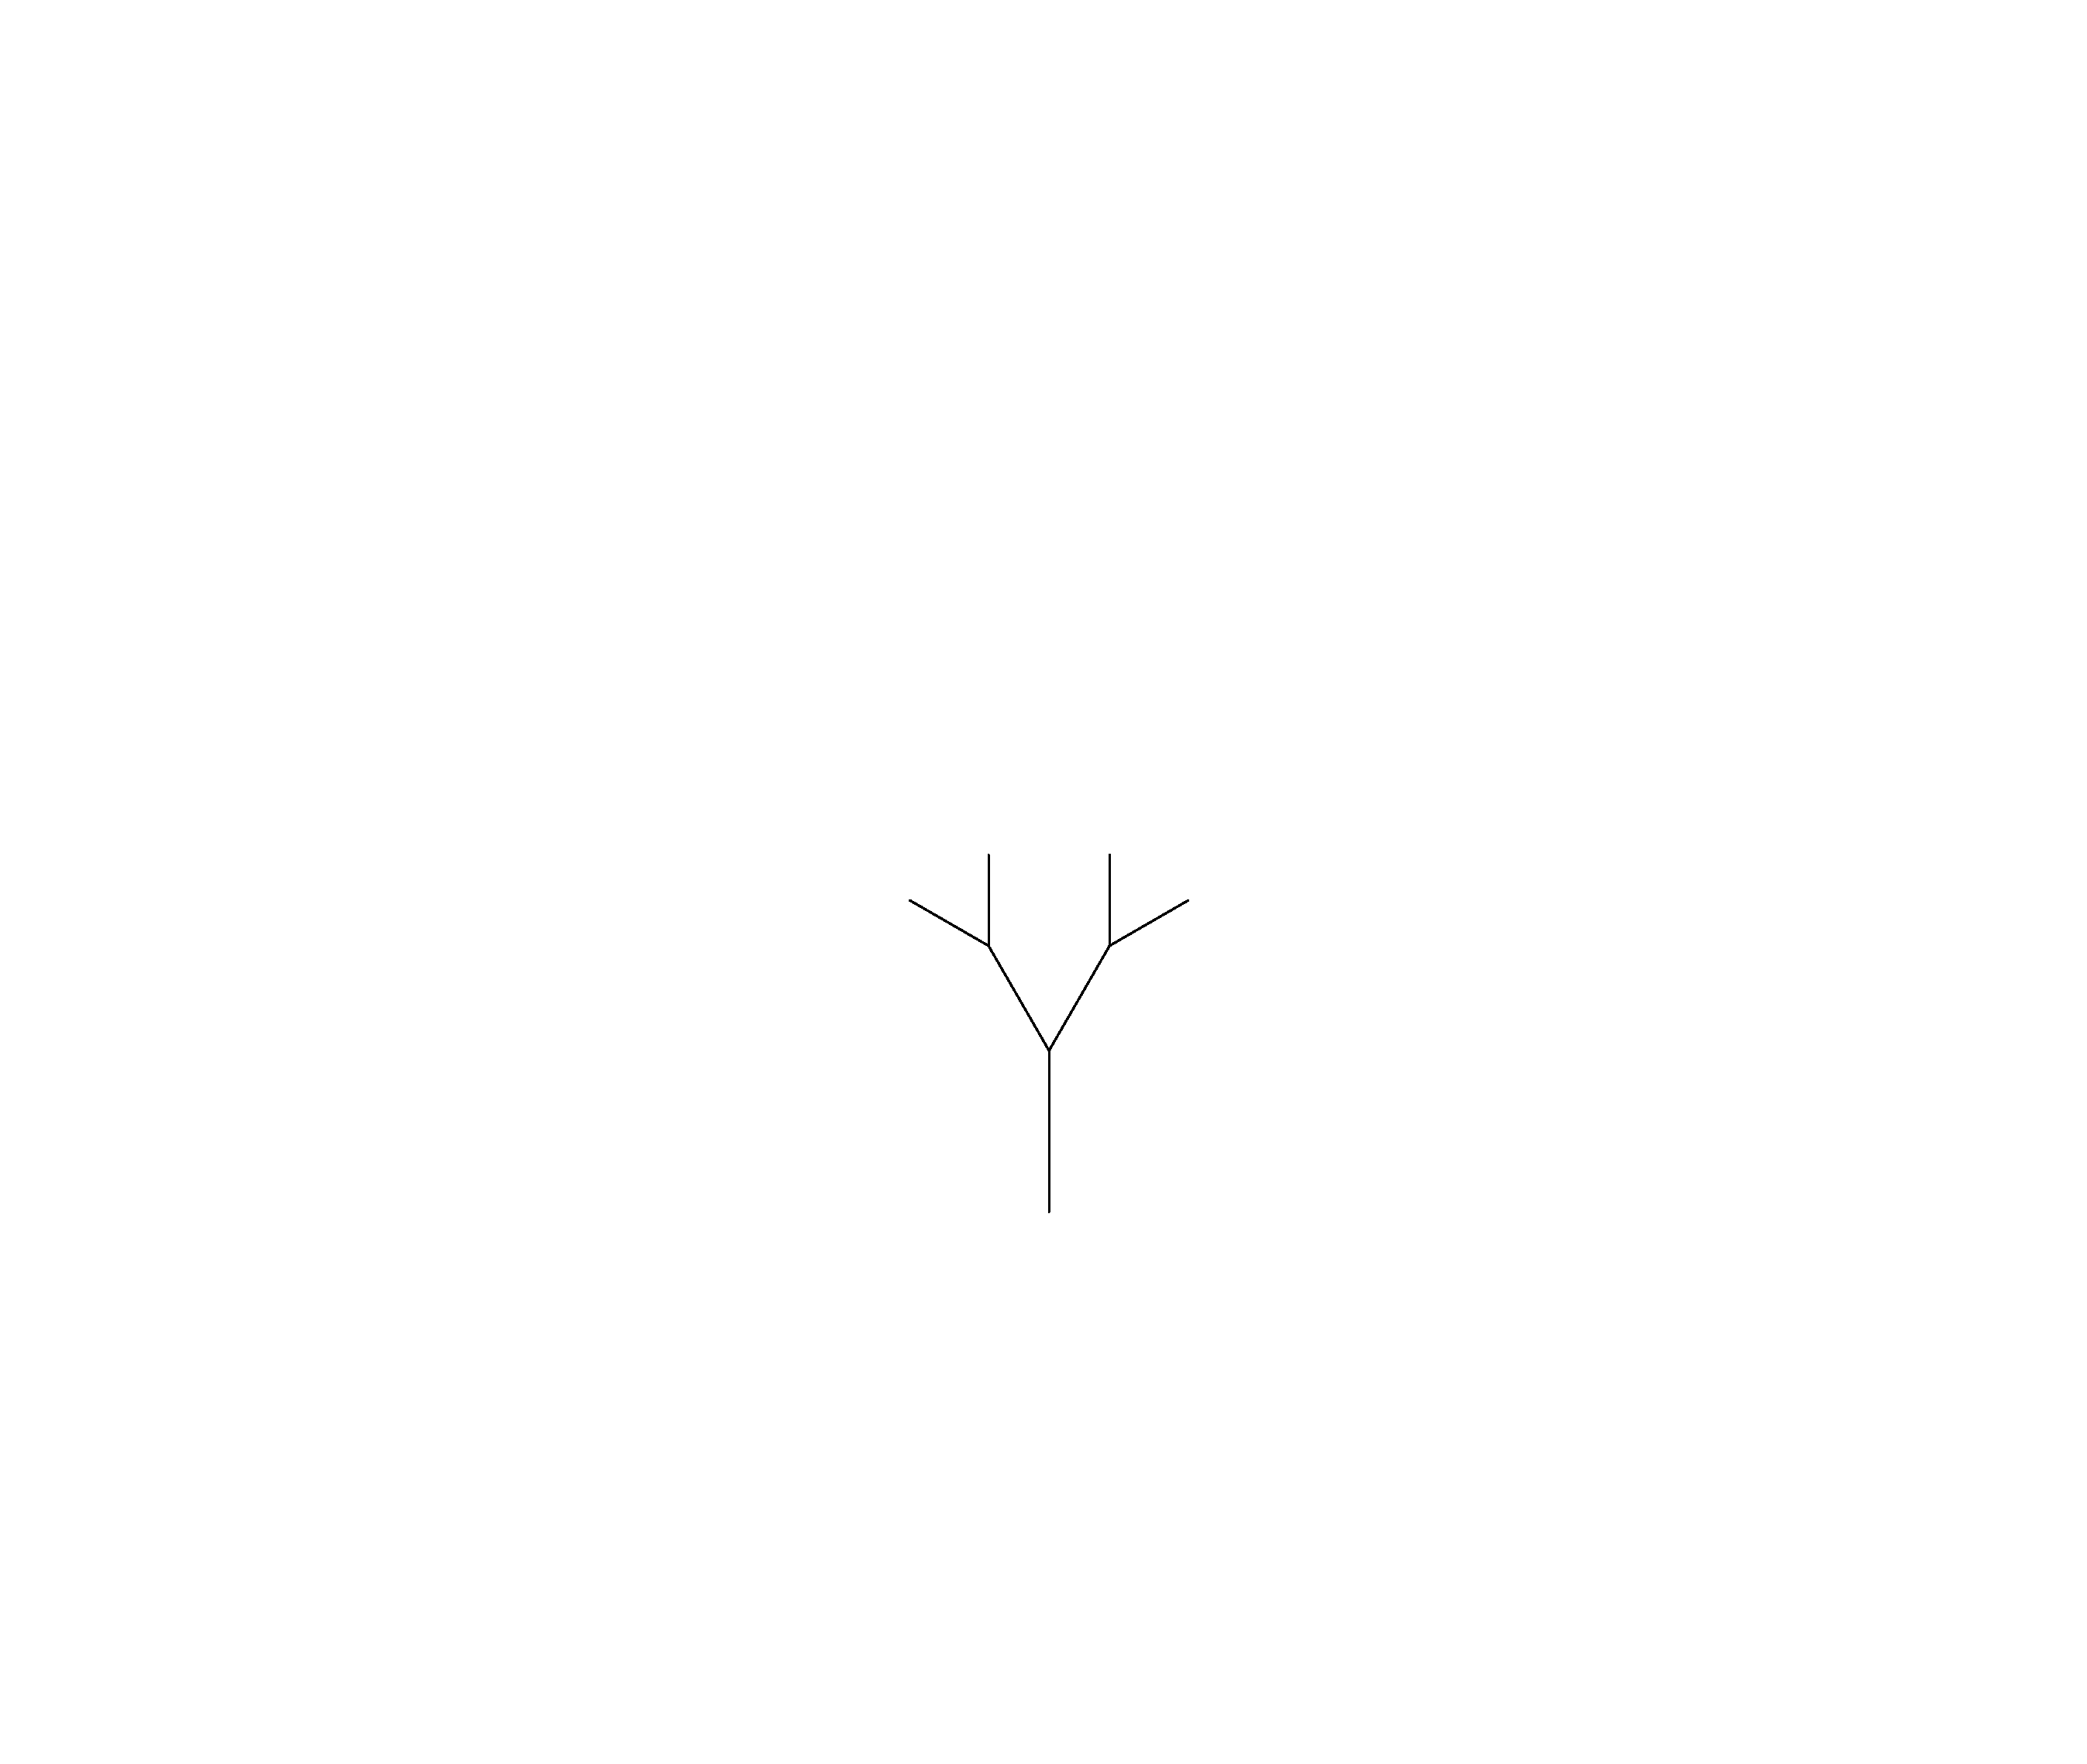
\includegraphics[trim=450 300 450 375,height=3.5cm]{3.eps}
}

\bigskip
\bigskip

4 ~
\fbox{
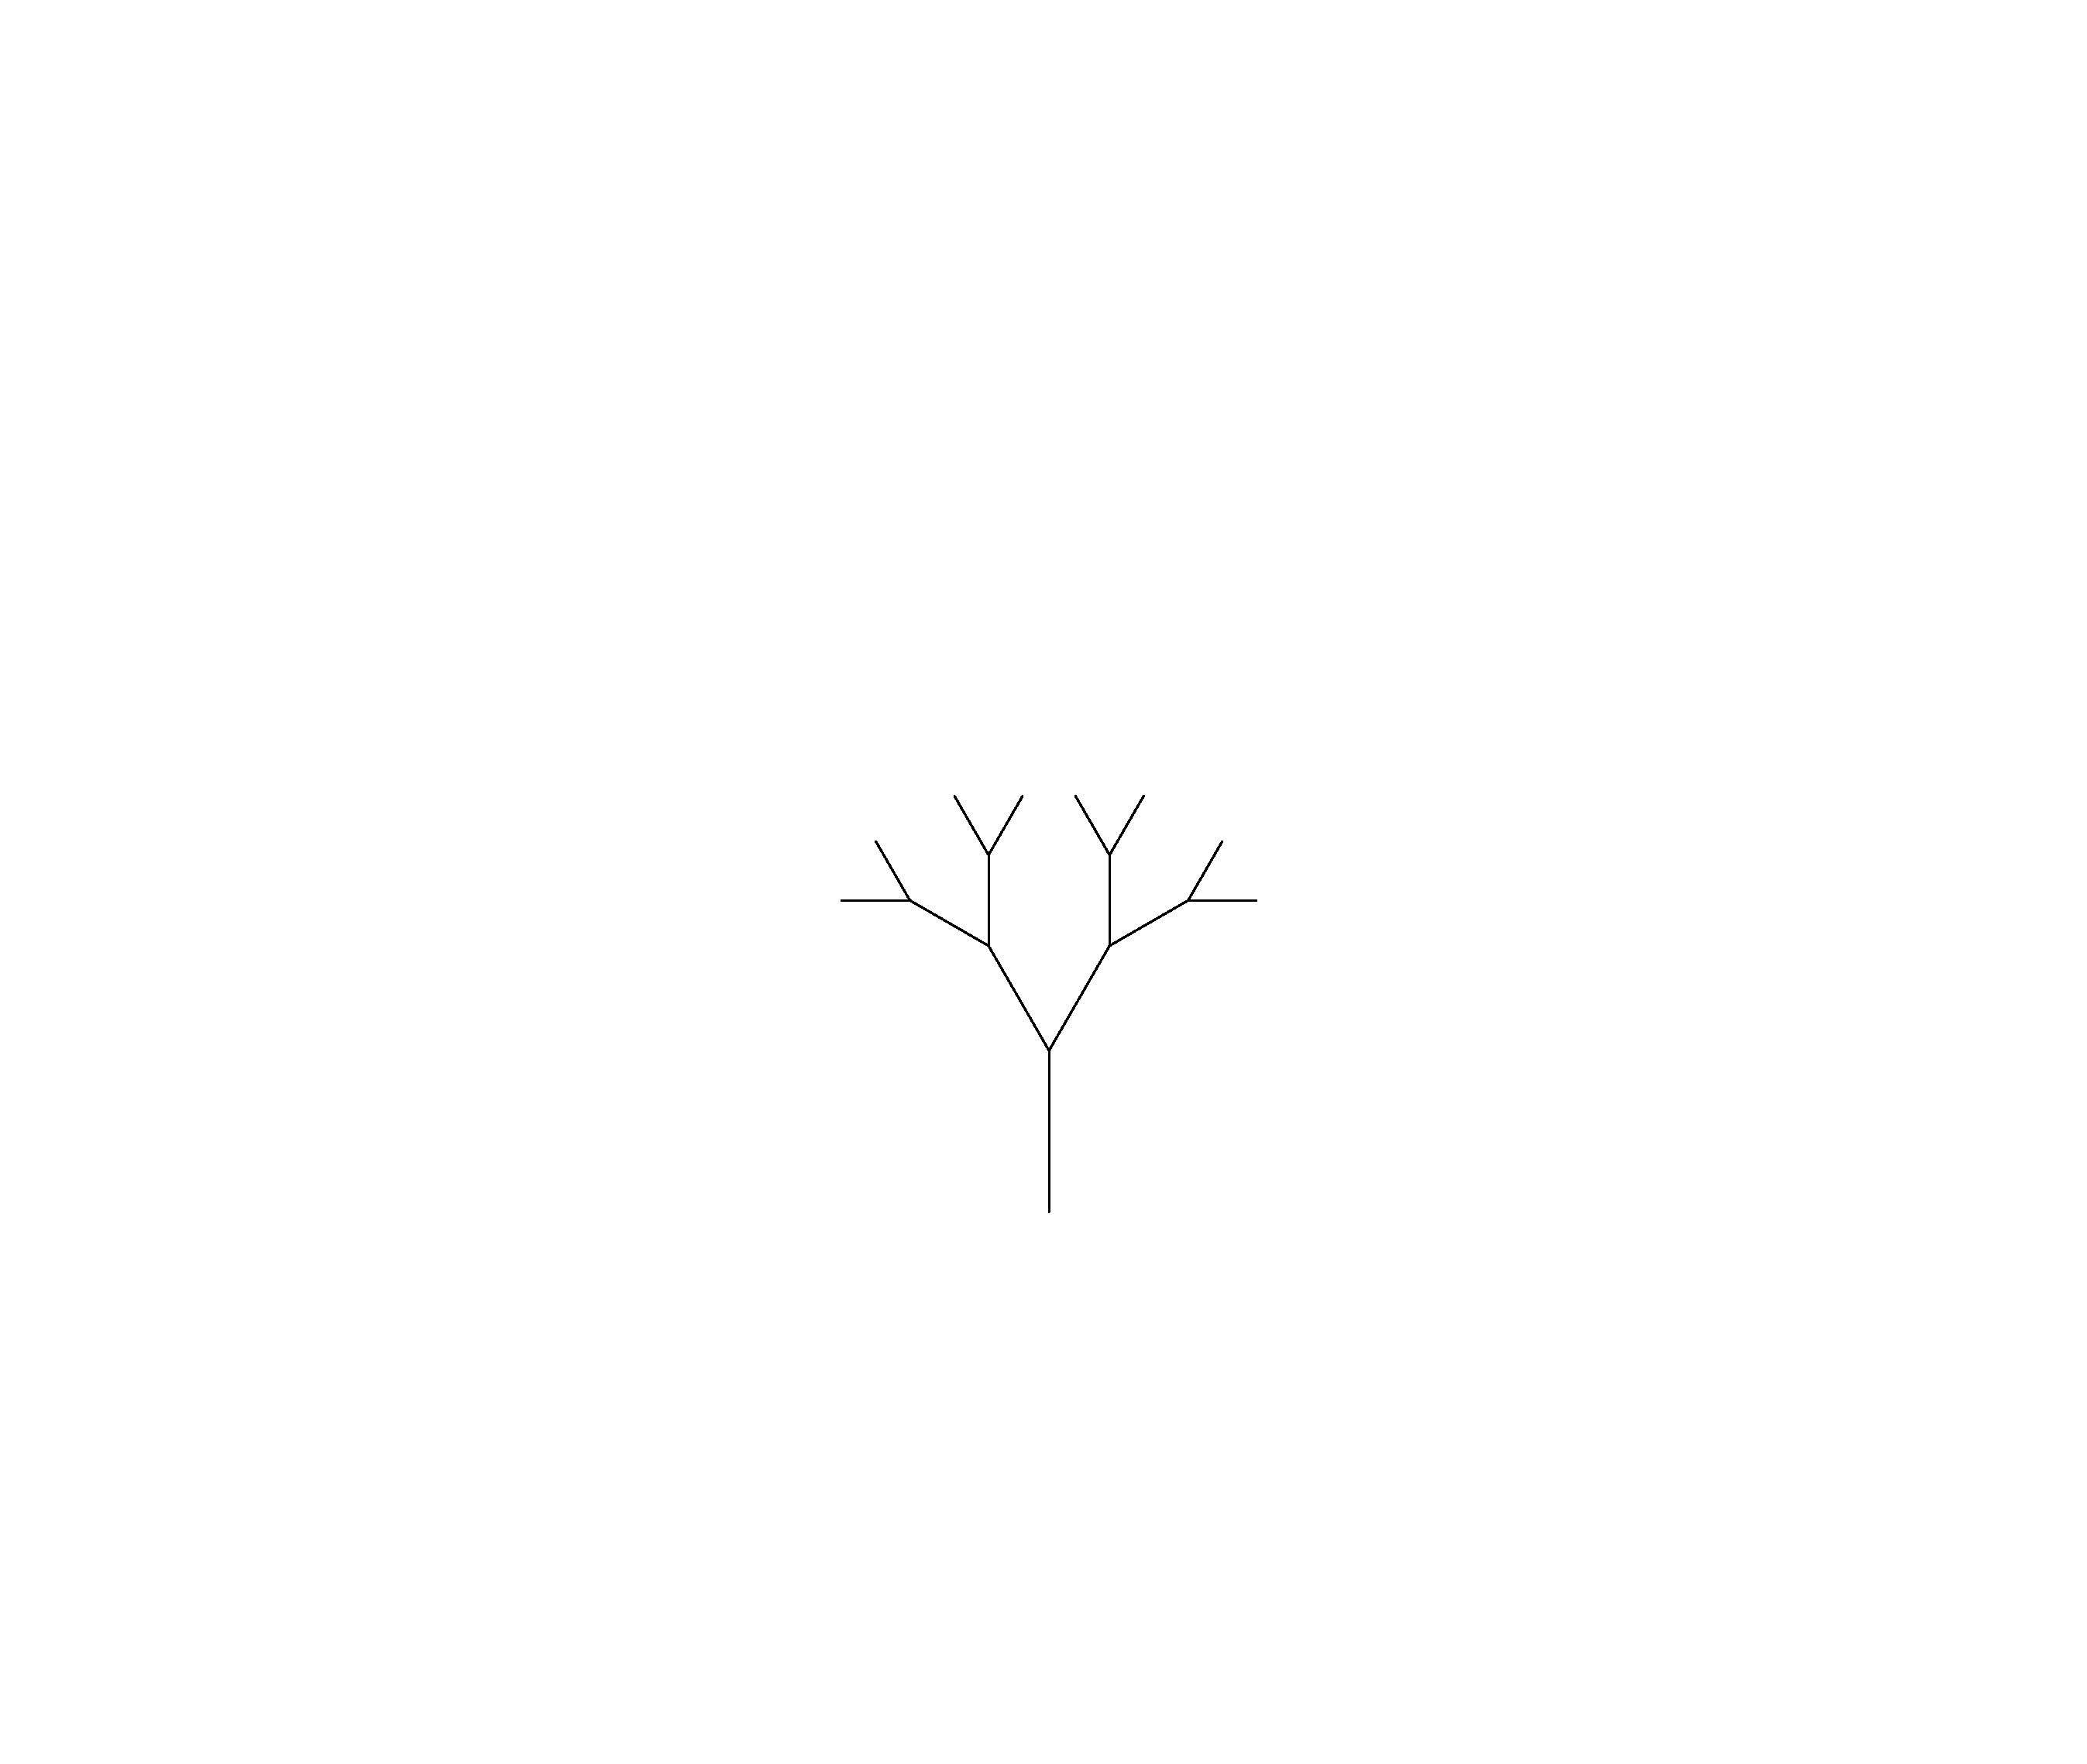
\includegraphics[trim=450 300 450 375,height=3.5cm]{4.eps}
}
\qquad
5 ~
\fbox{

\includegraphics[trim=450 300 450 375,height=3.5cm]{5.eps}
}
\qquad
6 ~
\fbox{

\includegraphics[trim=450 300 450 375,height=3.5cm]{6.eps}
}
\end{center}

\mysection{Entrada}

A l'entrada, es dónen tres valors: un natural $n$ amb el nombre de nivells de
l'arbre, un real positiu $d$ amb la seva mida, i un real $\alpha$ amb l'angle
(en graus) entre les seves branques.

\mysection{Sortida}

El programa ha de dibuixar un arbre d'$n$ nivells,
mida $d$ i angle $\alpha$.

\bigskip

\begin{multicols}{2}\raggedcolumns
\mysection{Exemple d'entrada 1}

\begin{verbatim}
4
100
30
\end{verbatim}

\columnbreak

\mysection{Exemple de sortida 1}

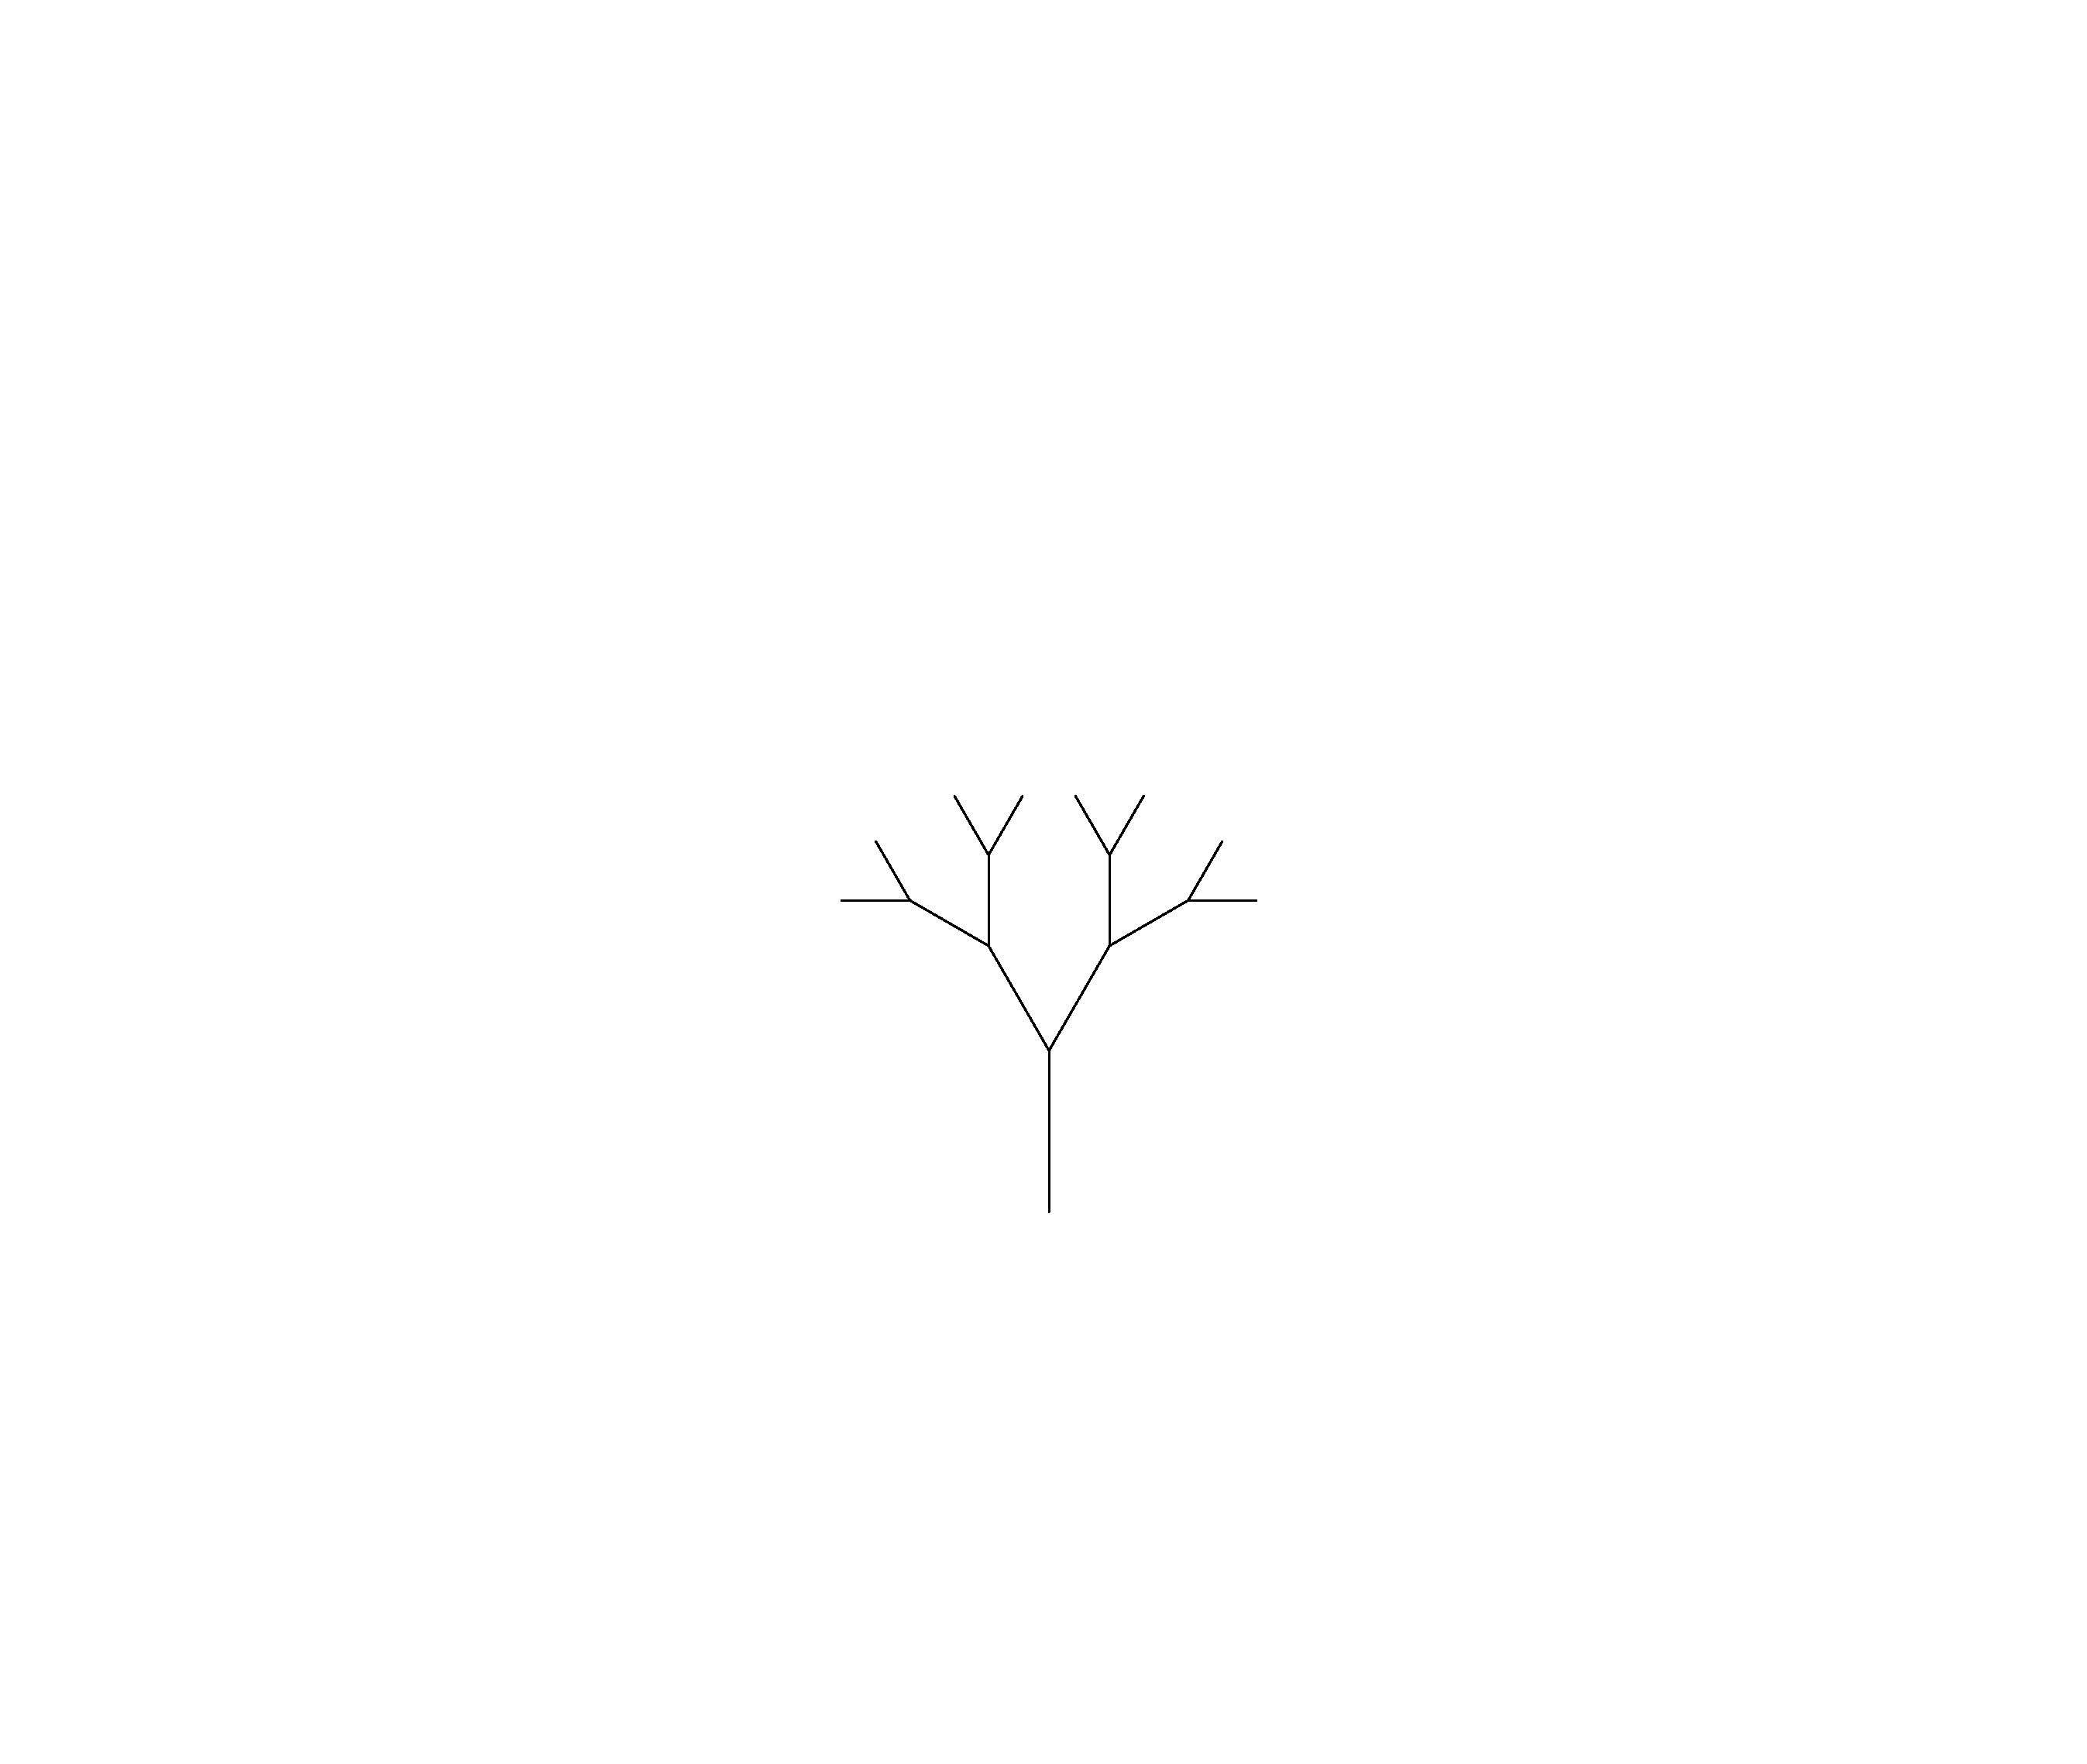
\includegraphics[trim=450 300 450 375,height=3.5cm]{4.eps}

\end{multicols}

\begin{multicols}{2}\raggedcolumns
\mysection{Exemple d'entrada 2}

\begin{verbatim}
5
200
90
\end{verbatim}


\columnbreak
\mysection{Exemple de sortida 2}

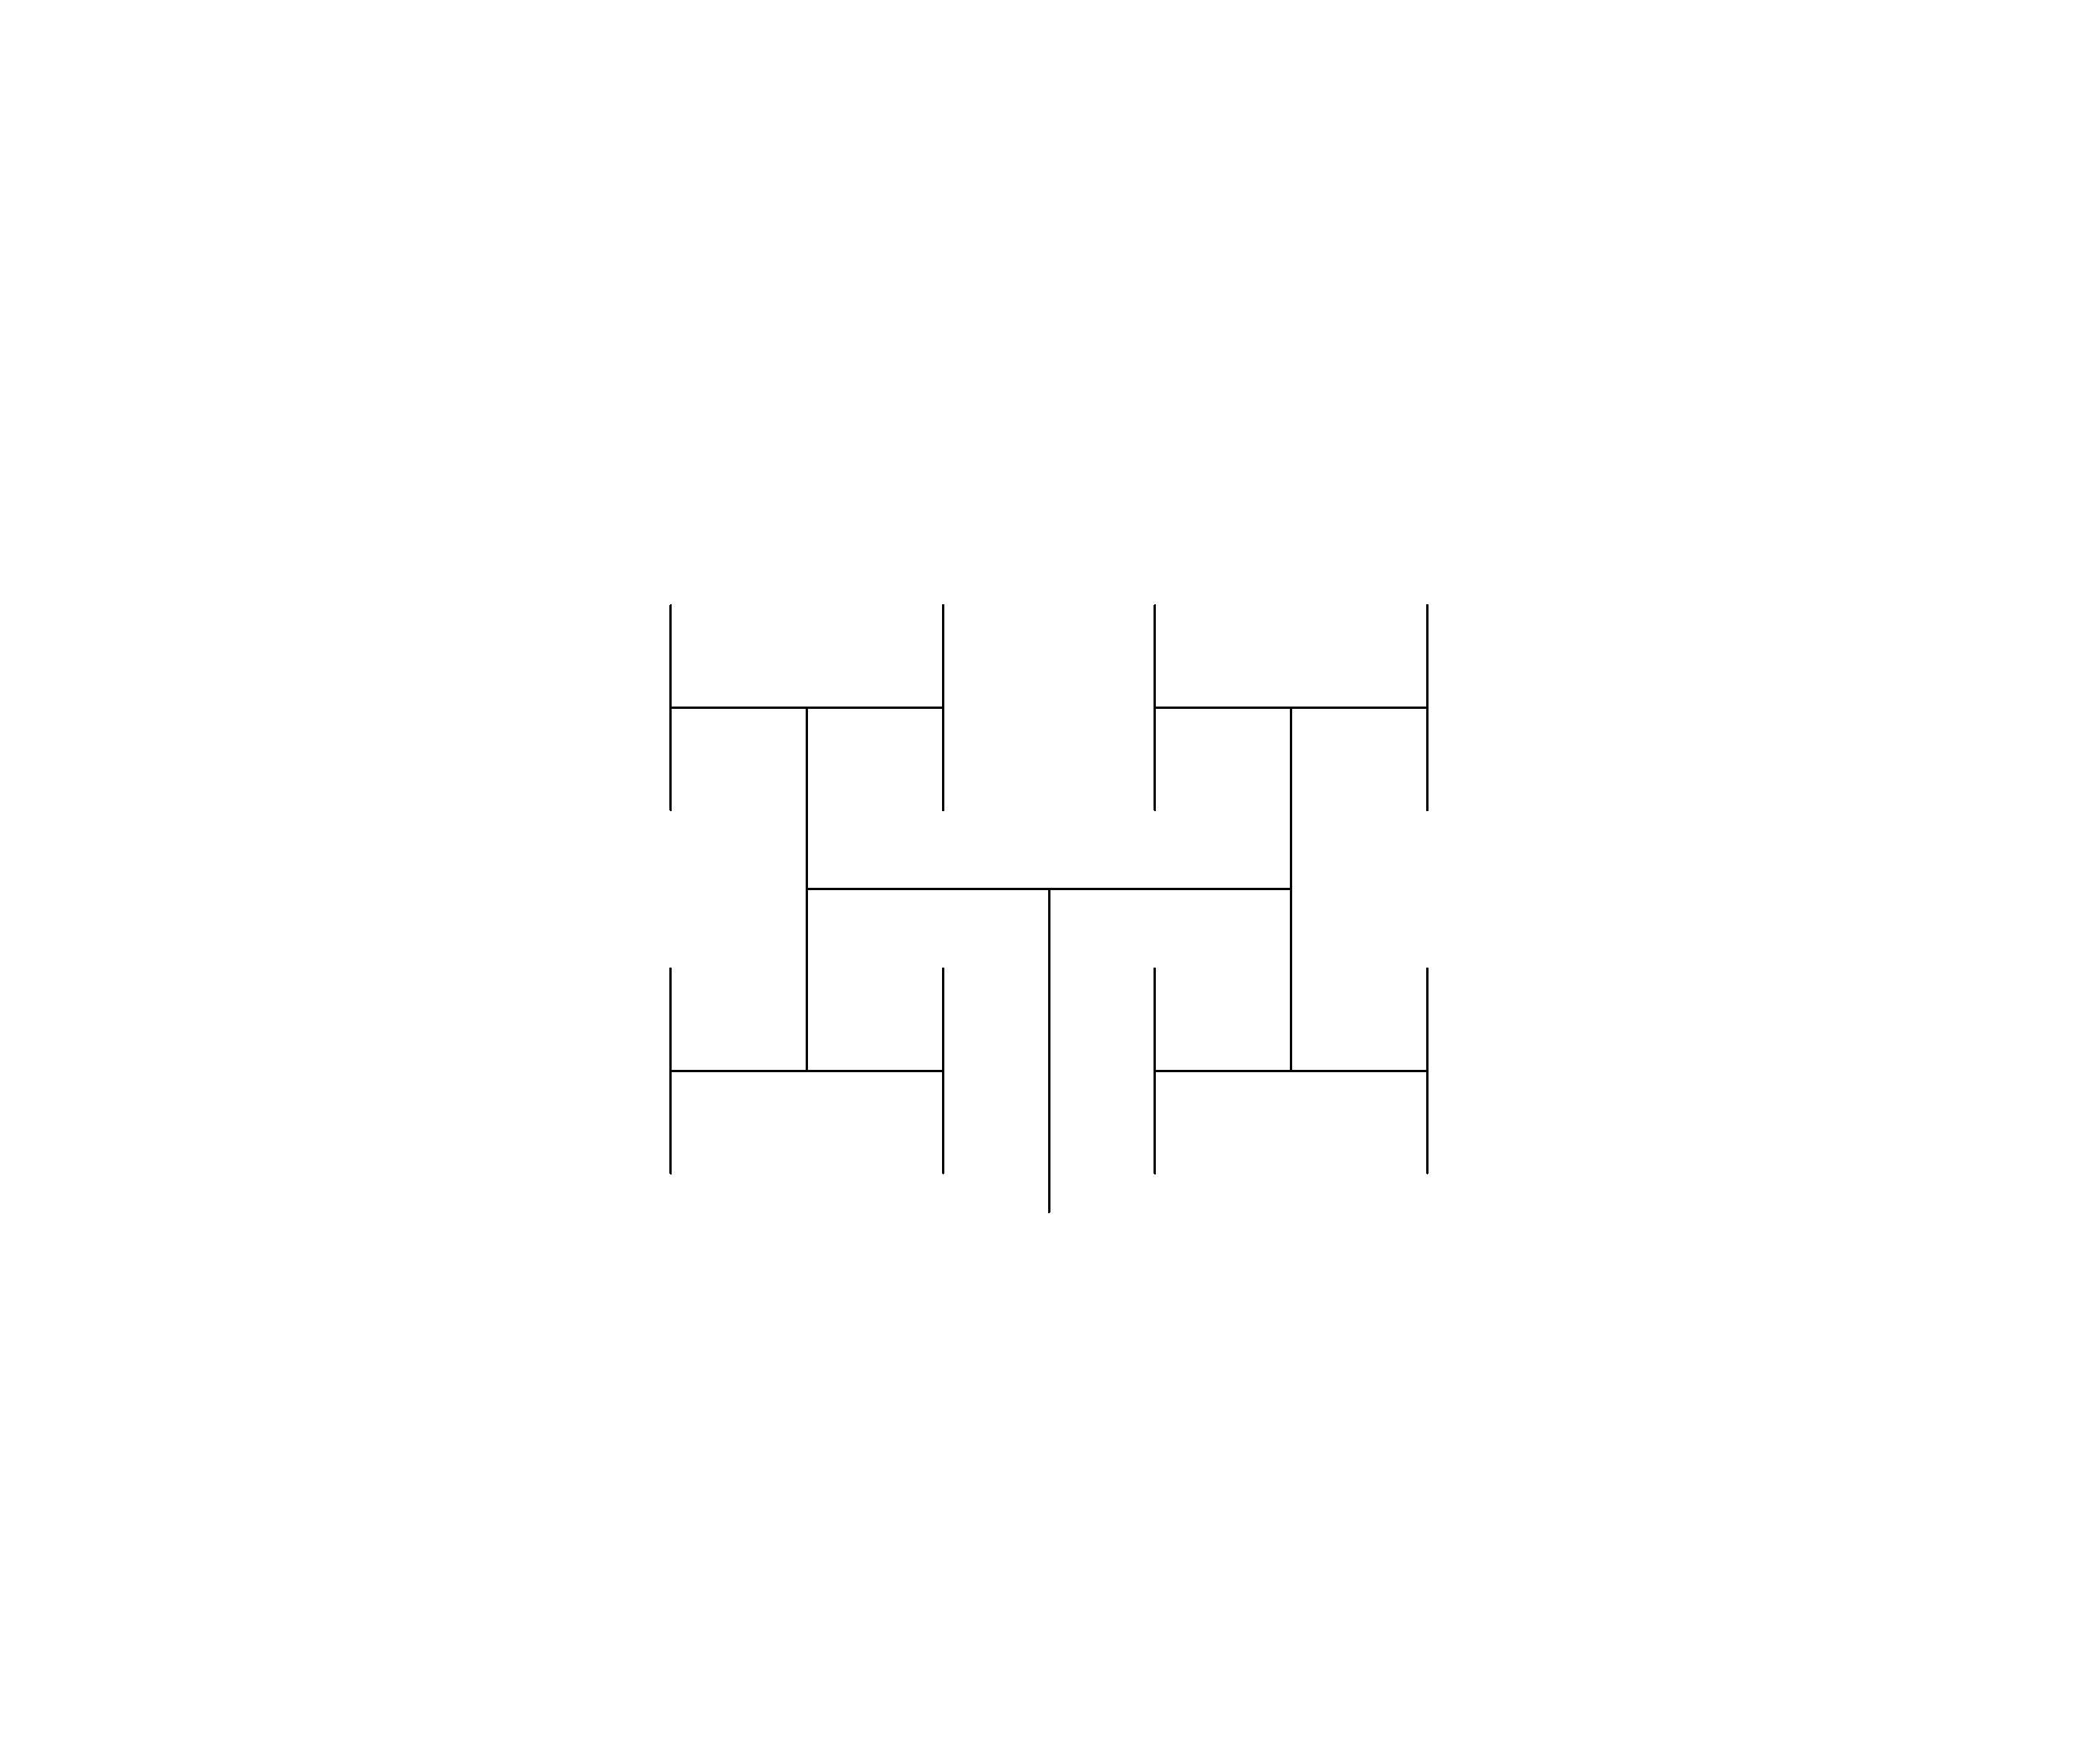
\includegraphics[trim=400 300 400 375,height=3.5cm]{sample2.eps}


\end{multicols}


\mysection{Recordatori}

Recordeu que Python ofereix un mòdul \texttt{turtle} que permet pintar images
amb una tortuga que es desplaça. Les úniques operacions que us calen són
\texttt{turtle.forward(d)} que avança la tortuga \texttt{d} unitats,
\texttt{turtle.backward(d)} que recula la tortuga \texttt{d} unitats,
\texttt{turtle.right(a)} que gira la tortuga \texttt{a} graus a la dreta i
\texttt{turtle.left(a)} que gira la tortuga \texttt{a} graus a l'esquerra.

\bigskip

Per exemple, aquest programa pinta un aborrit quadrat:

\begin{small}
\begin{verbatim}
import turtle
import jutge

d = jutge.read(float)
for i in range(4):
    turtle.forward(d)
    turtle.right(90)
\end{verbatim}
\end{small}

\mysection{Important}

Aquest problema no té jocs de proves al Jutge. Per tant, qualsevol solució serà
acceptada: semàfor verd! Això no vol dir que sigui bona ni dolenta, el vostre
professor ho corregirà.
